\section{Self-Supervised Learning: Wav2Vec 2.0}

\begin{frame}[allowframebreaks]{Wav2Vec 2.0}
    \begin{itemize}
        \item Proposed by Baevski et al. (2020): self-supervised learning for speech representation, the speech counterpart of BERT-style pretraining.
        \item \textbf{Architecture:} a CNN encoder turns the raw waveform into latent representations $z_t$; a transformer produces context representations $c_t$; a quantization module gives discrete targets $q_t$.
        \item \textbf{Pretraining:} mask spans of the latent sequence and train contrastively to pick the true quantized target among distractors, on unlabeled audio alone.
    \end{itemize}
    \framebreak
    \begin{figure}[h]
        \centering
        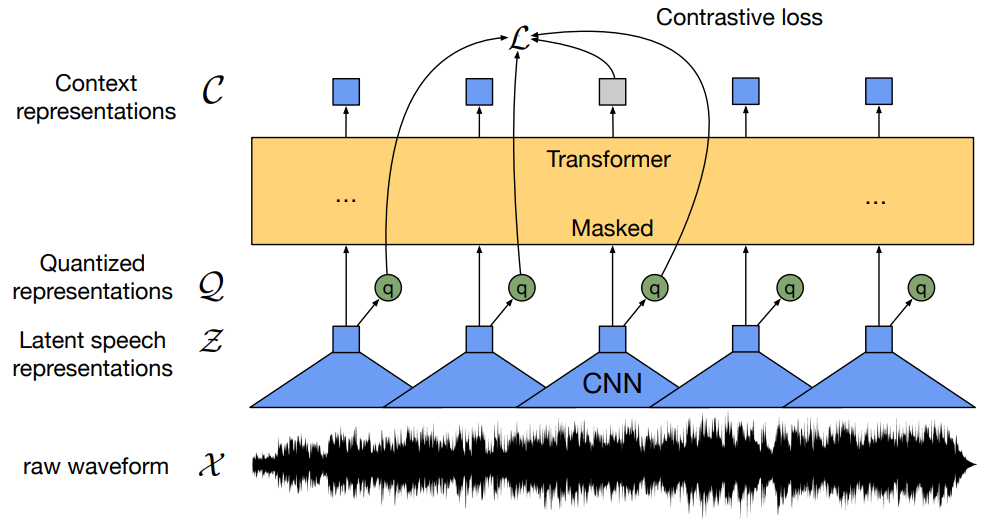
\includegraphics[width=\textwidth,height=0.55\textheight,keepaspectratio]{images/audio-nlp/wav2vec2-overview.png}
        \caption*{\scriptsize Source: Baevski et al., ``wav2vec 2.0: A Framework for Self-Supervised Learning of Speech Representations'', NeurIPS 2020, Fig.~1.}
    \end{figure}
\end{frame}
